% Options for packages loaded elsewhere
% Options for packages loaded elsewhere
\PassOptionsToPackage{unicode}{hyperref}
\PassOptionsToPackage{hyphens}{url}
\PassOptionsToPackage{dvipsnames,svgnames,x11names}{xcolor}
%
\documentclass[
  letterpaper,
  DIV=11,
  numbers=noendperiod]{scrartcl}
\usepackage{xcolor}
\usepackage{amsmath,amssymb}
\setcounter{secnumdepth}{-\maxdimen} % remove section numbering
\usepackage{iftex}
\ifPDFTeX
  \usepackage[T1]{fontenc}
  \usepackage[utf8]{inputenc}
  \usepackage{textcomp} % provide euro and other symbols
\else % if luatex or xetex
  \usepackage{unicode-math} % this also loads fontspec
  \defaultfontfeatures{Scale=MatchLowercase}
  \defaultfontfeatures[\rmfamily]{Ligatures=TeX,Scale=1}
\fi
\usepackage{lmodern}
\ifPDFTeX\else
  % xetex/luatex font selection
\fi
% Use upquote if available, for straight quotes in verbatim environments
\IfFileExists{upquote.sty}{\usepackage{upquote}}{}
\IfFileExists{microtype.sty}{% use microtype if available
  \usepackage[]{microtype}
  \UseMicrotypeSet[protrusion]{basicmath} % disable protrusion for tt fonts
}{}
\makeatletter
\@ifundefined{KOMAClassName}{% if non-KOMA class
  \IfFileExists{parskip.sty}{%
    \usepackage{parskip}
  }{% else
    \setlength{\parindent}{0pt}
    \setlength{\parskip}{6pt plus 2pt minus 1pt}}
}{% if KOMA class
  \KOMAoptions{parskip=half}}
\makeatother
% Make \paragraph and \subparagraph free-standing
\makeatletter
\ifx\paragraph\undefined\else
  \let\oldparagraph\paragraph
  \renewcommand{\paragraph}{
    \@ifstar
      \xxxParagraphStar
      \xxxParagraphNoStar
  }
  \newcommand{\xxxParagraphStar}[1]{\oldparagraph*{#1}\mbox{}}
  \newcommand{\xxxParagraphNoStar}[1]{\oldparagraph{#1}\mbox{}}
\fi
\ifx\subparagraph\undefined\else
  \let\oldsubparagraph\subparagraph
  \renewcommand{\subparagraph}{
    \@ifstar
      \xxxSubParagraphStar
      \xxxSubParagraphNoStar
  }
  \newcommand{\xxxSubParagraphStar}[1]{\oldsubparagraph*{#1}\mbox{}}
  \newcommand{\xxxSubParagraphNoStar}[1]{\oldsubparagraph{#1}\mbox{}}
\fi
\makeatother


\usepackage{longtable,booktabs,array}
\usepackage{calc} % for calculating minipage widths
% Correct order of tables after \paragraph or \subparagraph
\usepackage{etoolbox}
\makeatletter
\patchcmd\longtable{\par}{\if@noskipsec\mbox{}\fi\par}{}{}
\makeatother
% Allow footnotes in longtable head/foot
\IfFileExists{footnotehyper.sty}{\usepackage{footnotehyper}}{\usepackage{footnote}}
\makesavenoteenv{longtable}
\usepackage{graphicx}
\makeatletter
\newsavebox\pandoc@box
\newcommand*\pandocbounded[1]{% scales image to fit in text height/width
  \sbox\pandoc@box{#1}%
  \Gscale@div\@tempa{\textheight}{\dimexpr\ht\pandoc@box+\dp\pandoc@box\relax}%
  \Gscale@div\@tempb{\linewidth}{\wd\pandoc@box}%
  \ifdim\@tempb\p@<\@tempa\p@\let\@tempa\@tempb\fi% select the smaller of both
  \ifdim\@tempa\p@<\p@\scalebox{\@tempa}{\usebox\pandoc@box}%
  \else\usebox{\pandoc@box}%
  \fi%
}
% Set default figure placement to htbp
\def\fps@figure{htbp}
\makeatother





\setlength{\emergencystretch}{3em} % prevent overfull lines

\providecommand{\tightlist}{%
  \setlength{\itemsep}{0pt}\setlength{\parskip}{0pt}}



 


\KOMAoption{captions}{tableheading}
\makeatletter
\@ifpackageloaded{caption}{}{\usepackage{caption}}
\AtBeginDocument{%
\ifdefined\contentsname
  \renewcommand*\contentsname{Table of contents}
\else
  \newcommand\contentsname{Table of contents}
\fi
\ifdefined\listfigurename
  \renewcommand*\listfigurename{List of Figures}
\else
  \newcommand\listfigurename{List of Figures}
\fi
\ifdefined\listtablename
  \renewcommand*\listtablename{List of Tables}
\else
  \newcommand\listtablename{List of Tables}
\fi
\ifdefined\figurename
  \renewcommand*\figurename{Figure}
\else
  \newcommand\figurename{Figure}
\fi
\ifdefined\tablename
  \renewcommand*\tablename{Table}
\else
  \newcommand\tablename{Table}
\fi
}
\@ifpackageloaded{float}{}{\usepackage{float}}
\floatstyle{ruled}
\@ifundefined{c@chapter}{\newfloat{codelisting}{h}{lop}}{\newfloat{codelisting}{h}{lop}[chapter]}
\floatname{codelisting}{Listing}
\newcommand*\listoflistings{\listof{codelisting}{List of Listings}}
\makeatother
\makeatletter
\makeatother
\makeatletter
\@ifpackageloaded{caption}{}{\usepackage{caption}}
\@ifpackageloaded{subcaption}{}{\usepackage{subcaption}}
\makeatother
\usepackage{bookmark}
\IfFileExists{xurl.sty}{\usepackage{xurl}}{} % add URL line breaks if available
\urlstyle{same}
\hypersetup{
  colorlinks=true,
  linkcolor={blue},
  filecolor={Maroon},
  citecolor={Blue},
  urlcolor={Blue},
  pdfcreator={LaTeX via pandoc}}


\author{}
\date{}
\begin{document}


\section{Skripsi dalam Kurikulum Fakultas
Psikologi}\label{skripsi-dalam-kurikulum-fakultas-psikologi}

Kurikulum pendidikan Fakultas Psikologi Universitas YARSI masih
menjadikan Skripsi sebagai syarat wajib kelulusan mahasiswa. Untuk dapat
mengerjakan skripsi, setiap mahasiswa perlu memahami informasi-informasi
administratif yang menyangkut MK Skripsi. Informasi ini mencakup beban
SKS, persyaratan akademik dan administrasi, serta prosedur dan alur
kerja pengerjaan skripsi. Diagram alir (flow chart) prosedur pengerjaan
skripsi dapat dilihat pada Gambar 1.

\subsection{Kedudukan Skripsi dan Bobot
SKS}\label{kedudukan-skripsi-dan-bobot-sks}

Skripsi memiliki kedudukan yang sama dengan mata kuliah lain, hanya
berbeda dalam bentuk, proses belajar-mengajar dan cara penilaiannya.
Bobot skripsi adalah 8 SKS, yang setara dengan kegiatan akademik setiap
minggu 40 jam. Selama satu semester, bobot MK Skripsi setara dengan 640
jam pembelajaran (16 pertemuan).

\subsection{Persyaratan Mata Kuliah
Skripsi}\label{persyaratan-mata-kuliah-skripsi}

\begin{enumerate}
\def\labelenumi{\arabic{enumi}.}
\item
  Persyaratan akademik

  Untuk menempuh mata kuliah skripsi, mahasiswa harus memenuhi
  persyaratan akademik sebagai berikut:

  \begin{enumerate}
  \def\labelenumii{\alph{enumii}.}
  \tightlist
  \item
    Telah lulus Mata Kuliah Seminar Proposal Skripsi (SPS) pada semester
    sebelumnya,
  \item
    Telah menyelesaikan SKS dalam jumlah tertentu sesuai prasyarat dari
    Ketua Program Studi/Wakil Dekan 1
  \end{enumerate}
\item
  Persyaratan administratif

  Untuk menempuh MK Skripsi, mahasiswa harus memenuhi persyaratan
  administratif sebagai berikut:

  \begin{enumerate}
  \def\labelenumii{\alph{enumii}.}
  \item
    Telah memenuhi persyaratan akademik, sebagaimana tertera pada poin 1
    di atas
  \item
    Memiliki KRS semester yang berjalan yang mencantumkan MK Skripsi dan
    telah ditandatangani oleh Dosen Pembimbing Akademik (DPA)
  \end{enumerate}
\end{enumerate}

\subsection{Waktu Pelaksanaan Mata Kuliah
Skripsi}\label{waktu-pelaksanaan-mata-kuliah-skripsi}

\subsubsection*{Batas Waktu Mata Kuliah
Skripsi}\label{batas-waktu-mata-kuliah-skripsi}
\addcontentsline{toc}{subsubsection}{Batas Waktu Mata Kuliah Skripsi}

Tidak ada batasan maksimal bagi mahasiswa untuk dapat melaksanakan dan
menyelesaikan skripsi. Mahasiswa dapat tetap mengambil MK Skripsi selama
memenuhi persyaratan administrasi perkuliahan secara umum (lihat Buku
Panduan Akademik untuk membaca persyaratan administrasi ini). Meskipun
demikian, waktu pelaksanaan MK Skripsi idealnya ditempuh dalam
selama-lamanya 2 (dua) semester. Setiap semesternya, mahasiswa wajib
mengisi Kartu Rencana Studi (KRS) untuk melakukan daftar ulang pada MK
Skripsi.

\subsubsection*{Perpanjangan Waktu Mata Kuliah
Skripsi}\label{perpanjangan-waktu-mata-kuliah-skripsi}
\addcontentsline{toc}{subsubsection}{Perpanjangan Waktu Mata Kuliah
Skripsi}

Apabila dalam jangka waktu 2 (dua) semester mahasiswa belum mampu
menyelesaikan skripsinya, maka waktu penyelesaian MK Skripsi dapat
diperpanjang hingga habis masa studi maksimum sesuai kebijakan Program
Studi Sarjana. Perpanjangan waktu MK Skripsi dapat dilakukan dengan
mencantumkan kembali MK Skripsi di KRS. Mahasiswa yang belum
menyelesaikan skripsi hingga habis masa studi maksimumnya akan
dinyatakan \emph{Drop Out} (DO).

\subsubsection*{Mengulang Sidang Ujian
Skripsi}\label{mengulang-sidang-ujian-skripsi}
\addcontentsline{toc}{subsubsection}{Mengulang Sidang Ujian Skripsi}

\begin{enumerate}
\def\labelenumi{\alph{enumi}.}
\tightlist
\item
  Mahasiswa yang dinyatakan tidak lulus pada sidang ujian skripsi wajib
  mengulang Sidang Ujian Skripsi dengan melakukan perbaikan pada skripsi
  dengan waktu selambat-lambatnya 30 hari (1 bulan kalender) sejak
  diselenggarakannya sidang skripsi mahasiswa yang bersangkutan.
\item
  Apabila dalam Sidang Ujian Skripsi mahasiswa dinyatakan lulus, tetapi
  pengumpulan perbaikan (revisi) skripsi melebihi 30 hari (1 bulan
  kalender) setelah penyelenggaraan sidang, maka kelulusan MK Skripsi
  mahasiswa dibatalkan dan mahasiswa diwajibkan untuk mengulang ujian
  sidang skripsi. Mahasiswa dapat mengajukan kembali Sidang Ujian
  Skripsi dalam waktu 14 hari kerja setelah tenggat waktu pengumpulan
  perbaikan skripsi sebelumnya. Mahasiswa dapat lulus pada semester
  berjalan apabila telah mengumpulkan perbaikan skripsi sebelum batas
  waktu yudisium yang telah ditentukan.
\item
  Mahasiswa yang tidak hadir dalam Sidang Ujian Skripsi yang telah
  dijadwalkan karena alasan apapun akan dinyatakan tidak lulus ujian dan
  menerima konsekuensi seperti telah dijelaskan pada poin a.
\end{enumerate}

\subsection{Prosedur dan Alur Kerja Mata Kuliah
Skripsi}\label{prosedur-dan-alur-kerja-mata-kuliah-skripsi}

\subsubsection*{Pengajuan dan
Pendaftaran}\label{pengajuan-dan-pendaftaran}
\addcontentsline{toc}{subsubsection}{Pengajuan dan Pendaftaran}

Langkah awal pengerjaan skripsi dimulai dari pengajuan atau pendaftaran
tema dan topik proposal penelitian di Mata Kuliah SPS. Terdapat dua
skema pendaftaran tema dan topik penelitian, yaitu skema penelitian
mandiri dan skema penelitian payung. Pada skema mandiri, mahasiswa
mengajukan tema dan topik penelitian sesuai dengan minat masing-masing.
Sedangkan, pada skema payung, tema dan topik penelitian ditentukan oleh
dosen koordinator penelitian dari setiap payung penelitian. Setiap
mahasiswa dapat mengajukan atau mendaftar paling banyak dua tema
penelitian saat pendaftaran proposal penelitian, baik itu pada skema
mandiri maupun skema payung.

Skema payung bersifat rekrutmen terbuka, yang berarti seluruh mahasiswa
memiliki hak untuk mendaftar selama memenuhi persyaratan yang ditetapkan
oleh dosen koordinator penelitian payung. Namun, kuota mahasiswa
bimbingan pada skema payung terbatas, sehingga dosen koordinator
penelitian payung perlu melakukan seleksi terhadap mahasiswa yang
mendaftar. Mahasiswa yang mendaftar skema payung tetapi dinyatakan tidak
lolos seleksi akan diminta untuk melakukan pengajuan tema skema
penelitian mandiri.

\subsubsection*{Bimbingan SPS}\label{bimbingan-sps}
\addcontentsline{toc}{subsubsection}{Bimbingan SPS}

Penentuan pembimbing SPS dan skripsi dilakukan oleh Wakil Dekan II
berdasarkan pembahasan di Komite Skripsi dan bersifat mutlak.
Penggantian pembimbing hanya dimungkinkan apabila (a) mahasiswa
mengajukan permohonan tertulis penggantian pembimbing, (b) dosen
pembimbing mengajukan permohonan tertulis penggantian mahasiswa
bimbingan, atau (c) dosen pemimbing berhalangan untuk melakukan
pembimbingan dalam waktu yang lebih dari 3 bulan, misalnya, dosen
menjalani tugas belajar. Proses penggantian pembimbing harus mengikuti
SOP yang telah ditetapkan. Proses bimbingan berlangsung selama semester
berjalan, baik itu secara daring maupun luring. Mahasiswa wajib mencatat
setiap proses bimbingan di log book bimbingan yang diparaf oleh
pembimbing. Waktu dan durasi bimbingan ditentukan oleh masing-masing
mahasiswa dan dosen pembimbing. Baik dosen ataupun mahasiswa diharapkan
hadir dalam proses bimbingan pada waktu yang telah ditentukan.

\subsubsection*{Ujian SPS}\label{ujian-sps}
\addcontentsline{toc}{subsubsection}{Ujian SPS}

Seperti halnya mata kuliah lain, evaluasi terhadap proses pembelajaran
di MK SPS dilakukan melalui mekanisme ujian, dalam hal ini berbentuk
ujian komprehensif. Ujian MK SPS terdiri dari Ujian Tengah Semester
(UTS) yang mencakup pengujian komprehensi mengenai Bab 1 proposal
penelitian dan Ujian Akhir Semester yang mencakup pengujian komprehensi
mengenai Bab 1 hingga Bab 3 proposal penelitian. Penguji UTS dan UAS MK
SPS terdiri dari satu orang dosen yang ditentukan oleh Wakil Dekan II
melalui pertimbangan Komite Skripsi. Setiap ujian memiliki komponen
penilaian masing-masing. Rubrik komponen penilaian UTS dapat dilihat di
Lampiran 1, sedangkan rubrik komponen penelitian UAS dapat dilihat di
Lampiran 2.

Kelulusan MK SPS ditentukan berdasarkan nilai ujian. Mahasiswa
dinyatakan lulus apabila memperoleh nilai huruf minimal C. Mahasiswa
yang dinyatakan tidak lulus wajib mengulang ujian MK SPS pada semester
berikutnya. Mahasiswa yang tidak lulus hanya perlu melakukan UAS pada
ujian berikutnya jika topik penelitiannya tidak berubah. Apabila
mahasiswa yang tidak lulus ingin mengajukan permohonan penggantian topik
atau judul penelitian, maka ia harus mengulang proses pendaftaran dari
tahap awal.

Untuk dapat mengikuti ujian MKS SPS, terdapat sejumlah syarat yang harus
dipenuhi oleh mahasiswa, yaitu:

\begin{itemize}
\tightlist
\item
  Mengumpulkan naskah lengkap (Bab 1 untuk UTS; Bab 1-3 untuk UAS)
  kepada petugas Tata Usaha Bagian Akademik dalam format digital (format
  file .docx atau .pdf)
\item
  Menyerahkan bukti pemeriksaan kemiripan (similarity check) yang
  dilakukan melalui akun fakultas (oleh Wakil Dekan II) dengan tingkat
  kemiripan maksimal sebesar 25\%.
\item
  Menyerahkan lembar persetujuan pembimbing yang telah ditandatangani
  sebagai bukti bahwa pembimbing SPS menyetujui naskah telah layak untuk
  diuji.
\item
  Menyerahkan bukti kehadiran bimbingan setidak-tidaknya 7 (tujuh) kali
  untuk UTS dan 14 (empat belas) kali untuk UAS, termasuk kehadiran di
  kelas besar.
\end{itemize}

Jadwal ujian, baik UTS maupun UAS, ditetapkan oleh Wakil Dekan II dengan
mempertimbangkan periode UTS dan UAS MK lainnya. Durasi ujian selama 30
menit untuk UTS dan 60 menit untuk UAS. Penilaian UTS diberikan hanya
oleh dosen penguji, sedangkan UAS diberikan oleh penguji dan pembimbing.

\subsubsection*{Bimbingan Skripsi}\label{bimbingan-skripsi}
\addcontentsline{toc}{subsubsection}{Bimbingan Skripsi}

Mahasiswa yang dinyatakan lulus MK SPS dapat mendaftar MK Skripsi di
semester selanjutnya. Pada MK Skripsi, fokus utama adalah pengambilan
data penelitian berdasarkan proposal yang telah diuji dan penulisan
naskah skripsi. Selama menjalani MK Skripsi, mahasiswa diwajibkan terus
melakukan bimbingan dengan pembimbing skripsi dengan jumlah minimal 14
pertemuan.

Dalam perjalanannya, mahasiswa dibolehkan untuk mengubah variabel
penelitian yang diajukan dalam proposal berdasarkan sejumlah
pertimbangan, misalnya masukan dari penguji SPS. Dalam kasus ini,
mahasiswa perlu menjalani ujian kelayakan terhadap proposal
penelitiannya yang baru. Mekanisme ujian kelayakan ini serupa dengan UAS
MK SPS yang telah dijelaskan di bagian sebelumnya.

Pada masa bimbingan skripsi, Komite Skripsi akan menentukan dewan
pembimbing skripsi. Setiap mahasiswa akan dibimbing oleh dua pembimbing,
yaitu pembimbing ilmu dan pembimbing agama. Tugas utama pembimbing agama
adalah memberikan panduan dan arahan dalam penulisan skripsi terutama di
bagian relevansi topik penelitian dengan nilai-nilai dan ajaran agama
Islam. Selain itu, pembimbing agama juga memandu mahasiswa untuk
mengintegrasikan perspektif Agama Islam dalam menginterpretasikan hasil
dan temuan peneltiian yang akan dituangkan dalam Bab 5 Hasil Penelitian
Menurut Tinjauan Islam. Penggantian pembimbing, baik pembimbing ilmu dan
pembimbing agama, dapat diajukan oleh mahasiswa dengan menyerahkan surat
permohonan penggantian pembimbing, sesuai dengan SOP yang telah disusun.

\subsubsection*{Ujian Forum}\label{ujian-forum}
\addcontentsline{toc}{subsubsection}{Ujian Forum}

Setelah mahasiswa selesai menyusun naskah skripsi dengan lengkap, maka
ia dapat mengajukan pendaftaran ujian forum. Secara umum, ujian forum
merupakan ujian komprehensi yang bertujuan untuk mengevaluasi kelayakan
naskah skripsi untuk kemudian dipertahankan di sidang skripsi. Wakil
Dekan II menetapkan satu orang dosen yang akan berperan sebagai dosen
pembahas dalam ujian forum.

Untuk dapat mengikuti ujian forum, selain naskah skripsi, mahasiswa juga
perlu menyerahkan sejumlah dokumen lainnya, yaitu:

\begin{itemize}
\tightlist
\item
  Berkas kelayakan etik penelitian yang dikeluarkan oleh Lembaga
  Penelitian Universitas YARSI atau lembaga etik lainnya.
\item
  Bukti hasil pemeriksaan kemiripan (similarity check) yang dilakukan
  melalui akun fakultas dengan tingkat kemiripan maksimal sebesar 25\%
\item
  Bukti persetujuan ujian forum oleh pembimbing ilmu
\end{itemize}

Ujian forum dapat dilaksanakan secara terbuka maupun tertutup,
tergantung dari kesepakatan antara pembimbing skripsi dan dosen pembahas
dengan pertimbangan utama mengenai sensitivitas topik dan data
penelitian. Pada ujian forum terbuka, seluruh mahasiswa Fakultas
Psikologi berkesempatan untuk ikut hadir dan terlibat aktif dalam
pembahasan pada sesi tanya-jawab. Sedangkan, dalam ujian forum tertutup,
mahasiswa yang diuji hanya dapat mengundang dua orang mahasiswa lainnya
yang bertugas sebagai pembahas. Baik pada ujian forum terbuka maupun
tertutup, mahasiswa yang diuji diminta untuk mengundang satu orang
mahasiswa lainnya sebagai notulen sidang.

Durasi ujian forum adalah selama 90 menit, yang mencakup 15 menit
paparan hasil penelitian, 10-15 menit menit sesi tanya-jawab oleh
mahasiswa, dan 60-65 menit sesi tanya-jawab oleh dosen pembahas.
Penilaian ujian dilakukan oleh dosen pembahas (rubrik komponen penilaian
ujian forum dapat dilihat di Lampiran 3). Terdapat tiga kategori hasil
penilaian kelayakan, yaitu:

\begin{itemize}
\tightlist
\item
  Lolos dengan perbaikan minor. Mahasiswa diberikan waktu 14 hari
  kalender untuk mengumpulkan naskah revisi.
\item
  Lolos dengan perbaikan mayor. Mahasiswa diberikan waktu 30 hari
  kalender untuk mengumpulkan naskah revisi.
\item
  Tidak lolos. Mahasiswa wajib mengikuti ujian forum ulang.
\end{itemize}

Mahasiswa yang tidak dapat mengumpulkan naskah revisi pada waktu yang
telah ditentukan akan dinyatakan tidak lolos ujian forum. Sebagai
konsekuensinya, mahasiswa harus mengikuti ujian forum ulang. Naskah
revisi yang dikumpulkan harus menyertakan bukti persetujuan dari
pembimbing skripsi dan dosen pembahas ujian forum.

\subsubsection*{Sidang Skripsi}\label{sidang-skripsi}
\addcontentsline{toc}{subsubsection}{Sidang Skripsi}

Mahasiswa yang telah dinyatakan lolos ujian forum dan mengumpulkan
naskah revisi pada tenggat waktu yang diberikan dapat segera mengajukan
pendaftaran ujian sidang skripsi. Untuk dapat mengikuti ujian skripsi,
mahasiswa harus sudah dinyatakan lulus pada seluruh mata kuliah selain
Skripsi dan telah menyelesaikan seluruh administrasi keuangan. Penetapan
jadwal dan dewan penguji sidang skripsi ditentukan oleh Wakil Dekan II
selaku ketua Komite Skripsi. Dewan Penguji terdiri dari satu orang dosen
penguji yang bertindak sebagai Ketua Dewan Penguji, dosen pembimbing
ilmu sebagai Anggota Dewan Penguji I sekaligus notulen sidang, dan dosen
pembimbing agama sebagai Anggota Dewan Penguji II.

Sidang skripsi berlangsung selama 90 menit, yang mencakup 15 menit
paparan skripsi oleh mahasiswa dan 75 menit sesi tanya-jawab oleh Dewan
Penguji. Penilaian MK Skripsi terdiri dari dua komponen utama, yaitu
performa mahasiswa selama bimbingan skripsi dan performa mahasiswa dalam
penulisan dan paparan skripsi (dalam sidang skripsi). Penilaian komponen
performa bimbingan diberikan oleh pembimbing ilmu dan pembimbing agama,
sedangkan komponen performa penulisan dan paparan skripsi dinilai oleh
seluruh Dewan Penguji. Rubrik komponen penilaian sidang skripsi dapat
dilihat di Lampiran 4.

Mahasiswa dinyatakan lulus ujian skripsi jika memperoleh nilai huruf
serendah-rendahnya B-. Mahasiswa yang memperoleh nilai huruf lebih
rendah dari B- dinyatakan tidak lulus dan wajib mengikuti sidang skripsi
ulang. Mahasiswa yang telah dinyatakan lulus sidang skripsi akan diminta
untuk menandatangani di atas meterai surat pernyataan yang pada intinya
menyatakan kesanggupan untuk mengumpulkan naskah revisi skripsi
selambat-lambatnya 30 hari kalender dari tanggal sidang skripsi. Surat
pernyataan tersebut juga memuat sejumlah konsekuensi yang akan dihadapi
oleh mahasiswa apabila tidak dapat mengumpulkan revisi skripsi sebelum
tenggat waktu yang ditentukan, termasuk di antaranya adalah pembatalan
kelulusan sidang skripsi dan kewajiban membayar penuh biaya pendidikan
untuk satu semester berikutnya.

\subsubsection*{Yudisium}\label{yudisium}
\addcontentsline{toc}{subsubsection}{Yudisium}

Yudisium adalah penentuan nilai atau kelulusan suatu ujian sarjana di
perguruan tinggi. Seluruh mahasiswa yang telah dinyatakan lulus sidang
skripsi dan mengumpulkan revisinya akan diinformasikan mengenai status
dan predikat kelulusannya dalam acara yudisium. Yudisium biasanya
diselenggarakan di pengujung semester berjalan. Dalam acara ini juga
diumumkan mengenai mahasiswa yang memperoleh penghargaan Skripsi Terbaik
yang ditetapkan berdasarkan nilai ujian skripsi. Yudisium merupakan
tahapan akademik terakhir sebelum wisuda.

\afterpage{%
  \clearpage
  \thispagestyle{empty}
  \begin{center}
    \includegraphics[width=\paperwidth,height=\paperheight,keepaspectratio]{1_1_alurskripsi.jpg}
  \end{center}
  \clearpage
}

\begin{figure}[H]

{\centering \pandocbounded{\includegraphics[keepaspectratio]{images/1_1_alurskripsi.png}}

}

\caption{Alur Kerja Mata Kuliah Skripsi}

\end{figure}%




\end{document}
